% arara: xelatex: {synctex: true}
% arara: indent: {overwrite: yes}
\documentclass[]{IMTexam}

\usepackage[enums]{IMTtikz}

\DeclareSIUnit{\parsec}{pc}
\DeclareSIUnit{\solarmass}{M_\odot}
\DeclareSIUnit{\ano}{ano}
%\DeclareSIUnit{\dia}{dia}

\givecredits
\author{Isabella B.}
\USPN{11810773}
\date{}
\lecture{Física I} % disciplina
\lcode{4302111}
\hwtype{Resolução} % o que é
\examname{Provinha IX} % prova

\begin{document}

\maketitle

\begin{questions}

	\titledquestion{Matéria escura em aglomerados de galáxias} \label{ques:q1}

	Em 1933, o astrônomo suíço-americano Fritz Zwicky, baseando-se em medidas publicadas por Edwin Hubble e Milton Humason, em 1931, foi o primeiro astrônomo a trazer provas convincentes acerca da existência da chamada \textit{matéria escura}%
	\footnote{Apesar do termo ter-se popularizado com o trabalho de Zwicky, ele não foi o primeiro a introduzir o termo em context astronômico. Em 1906, Henri Poincaré já havia discutido a possibilidade da existência de “matière obscure” dentro da nossa própria galáxia [Poincaré, H. “The Milky Way and the Theory of Gases”, Popular Astronomy, v. 14, p.475-488, 1906]. Se você não sabia, o Teorema do Virial foi derivado pela primeira vez no contexto da teoria cinética dos gases. Ele estava sendo utilizado por Kelvin (sim, o cara da termodinâmica) na tentativa de estimar a densidade de matéria na Via Láctea.}. Vamos entender como isso aconteceu.

	\begin{figure}[H]
		\centering
		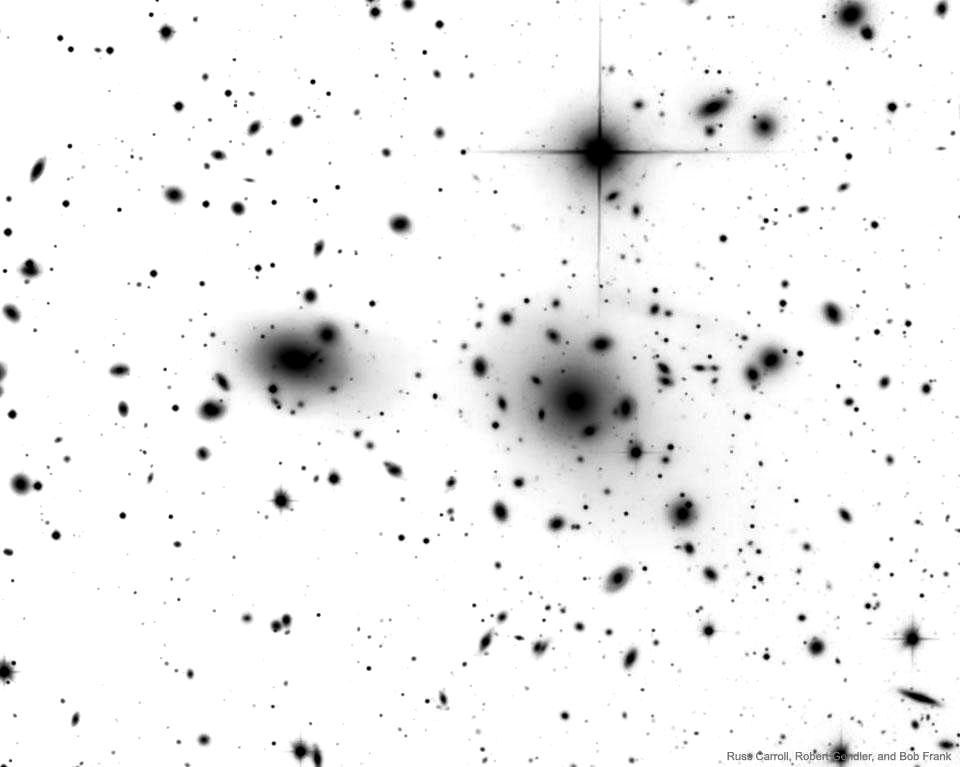
\includegraphics[width=0.4\linewidth]{screenshot001}
		\caption{Aglomerado de galáxias \textit{Coma}. Quase todo objeto mostrado na imagem é uma galáxia e é um dos aglomerados mais densos hoje conhecido, contendo milhares de galáxias. Cada uma das galáxias possui bilhões de estrelas. Ainda que próximo de nós se comparado à distância de outros aglomerados conhecidos, a luz de Coma demora cerca de centenas de milhares de anos para chegar até nós. Ainda mais: o aglomerado é tão grande que a luz demora milhões de anos para ir de um lado ao outro do aglomerado. [Crédito: Russ Carroll, Robert Gendler, \& Bob Franke; Dan Zowada Memorial Observatory]}
		\label{fig:fig1}
	\end{figure}

	Zwicky observou que a dispersão (desvio padrão) da componente da velocidade ao longo da linha de visada, também chamada de velocidade radial, de oito galáxias individuais no aglomerado é da ordem de $ \sigma_r=\sqrt{\<v_r^{2}>-\<v_r>^{2}}\sim 10^{3}\,\si{\kilo\meter\per\second} $. Esta medida nos da uma ótima estimativa da energia cinética do sistema. Contudo, a quantidade de matéria e gás visíveis no aglomerado não são capazes de produzir atração gravitacional suficiente para manter o sistema ligado! Tal fato já havia sido notado por Hubble e Humason, mas foi Zwicky quem aplicou o teorema do virial para estimar a massa do aglomerado (até onde sabemos).
	\begin{unindent}[start=0]
		\item \textbf{Unidades:} Utilizaremos o parsec para medir distâncias. Tal unidade é comumente adotada em cosmologia e astronomia galáctica e extragaláctica:
		\[ \SI{1}{\parsec}\approx \SI{3e13}{\kilo\meter} \]
		Também trabalharemos com anos (quanto vale um ano em segundos?). Para a sua sanidade, escreva a velocidade das galáxias nessas unidades (\si{\parsec\per\ano}) e trabalhe com essas unidades no que segue!

		\item Primeiro, vamos entender por que é razoável utilizar o teorema do virial nessa situação. Assuma que o raio e idade do aglomerado são da ordem de $ \sim\SI{1.5}{\mega\parsec} $, onde $ \SI{1}{\mega\parsec}=\SI{1e6}{\parsec} $, e $ \sim10^{10} $ anos, respectivamente. Estime quantos anos leva para uma galáxia atravessar o aglomerado e, com isso, estime quantas vezes cada galáxia pode cruzar, em média, o aglomerado. Argumente porque podemos supor que o aglomerado de Coma encontra-se em equilíbrio e, portanto, podemos utilizar o teorema do virial.

		\begin{solution}
			Sendo a velocidade radial em relação à um observador na Terra, podemos estabelecer que a medida de dispersão $ \sigma_r $ das oito galáxias do aglomerado consideradas no problema é uma boa medida da velocidade relativa média das galáxias em relação a Coma.

			Convertendo a medida de $ \sigma_r $ dada, temos:
			\[ \sigma_r=\dfrac{\SI{1e3}{\kilo\meter}}{\SI{1}{\second}}\cdot\dfrac{\SI{1}{\parsec}/\SI{3e13}{\kilo\meter}
				}{\del{\SI{1}{\ano}/365\,\text{dias}}\cdot
					\del{1\,\text{dia}/\SI{24}{\hour}}\cdot
					\del{\SI{1}{\hour}/\SI{60}{\minute}}\cdot
					\del{\SI{1}{\minute}/\SI{60}{\second}}}\approx\SI{1e-3}{\parsec\per\ano} \]
			Dessa forma, podemos estimar que uma galáxia qualquer leva
			\[ \dfrac{2\cdot\SI{1.5e6}{\parsec}}{\SI{1e-3}{\parsec\per\ano}}=\num{3e9}\,\text{anos} \]
			para cruzar o aglomerado, e, portanto, cruzou-o, em média $ \num{1e10}/\num{3e9}\approx \num{3.3} $ vezes.

			Dessa forma, assumindo que as galáxias tem idade aproximada à do aglomerado, podemos concluir que, na média de $ 10^{10} $ anos, todas as galáxias já puderam se locomover algumas vezes por toda a sua extensão, e que o sistema encontra-se em equilíbrio dinâmico, de tal forma que vale o teorema do virial.
		\end{solution}

		\item Vamos fazer então a aproximação da vaca esférica: trate o aglomerado como sendo uma esfera homogênea de massa $ M $ e raio $ R $. Mostre que a energia potencial total é dada por
		\[ u=-\dfrac{3}{5}\dfrac{G\,M^{2}}{R} \]

		\textit{Dica: considere a energia potencial gravitacional que uma casca esférica de espessura $ \dif r $ (qual é a massa $ m(r) $ da casca?) sente na presença de um núcleo esférico sólido de raio $ r $ e densidade $\rho$ constante (e qual é a massa $ M(r) $ do núcleo?).}

		\begin{solution}
			Sendo a energia potencial de uma massa $ m $ em relação a um ponto de massa $ M(r) $
			\[ U(r)=-\int_\infty^{r}\vec{F}(\vec{r'})\cdot\dif\vec{r'}=-\dfrac{G\,M(r)\,m}{r}, \]
			podemos tomar o diferencial $ \dif U $ em relação a uma massa $ \dif m $ e, daí, temos:
			\begin{align*}
				\dif U                   & =-\dfrac{G\,M(r)\,\dif m}{r}                                                                        \\
				\intertext{integrando de $ 0 $ à $ R $, temos}
				\int_{U(0)}^{U(R)}\dif U & =\int_{M(0)}^{M(R)}-\dfrac{G\,M(r)\,\dif m}{r}                                                      \\
				\intertext{aproximando o objeto como uma esfera, temos $ M(r)=\frac{4}{3}\pi\,\rho\,r^{3}\implies \dif m=4\pi\,\rho\,r^{2}\dif r $, portanto}
				U                        & =\int_{0}^{R}-\dfrac{G\del{\frac{4}{3}\pi\,\rho\,r^{3}}\del{4\pi\,\rho\,r^{2}\dif r}}{r}            \\
				                         & =-\dfrac{G\del{\frac{4}{3}\pi\,\rho\,r^{3}}\del{4\pi\,\rho\,r^{2}\dif r}}{r}\int_{0}^{R}r^{5}\dif r \\
				                         & =-\dfrac{16}{3}G\pi^{2}\,\rho^{2}\int_{0}^{R}r^{4}\dif r                                            \\
				                         & =-\dfrac{16}{3}G\pi^{2}\,\rho^{2}\eval{\del{\dfrac{1}{5}r^{5}}}_0^{R}                               \\
				                         & =-\dfrac{3}{5}\dfrac{G}{R}\del{\dfrac{4}{3}\pi\,\rho\,R^{3}}^{2}                                    \\
				U                        & =-\dfrac{3}{5}\dfrac{G\,M^{2}}{R}
			\end{align*}

			\hfill\qedsymbol
		\end{solution}

		\item Uma vez que você se convenceu que o sistema pode ser tratado como estando em equilíbrio, considere a energia cinética média, $ K=\frac{1}{2}M\<v^{2}> $, e utilize o teorema do virial para expressar a massa $ M $ do aglomerado em termos da média do raio $ R $ do aglomerado e do quadrado da velocidade tridimensional, $ \<v_{\textup{tot}}^{2}>=\<v_x^{2}+v_y^{2}+v_z^{2}> $.

		\begin{solution}
			Pelo teorema do virial, temos
			\begin{align}
				2\<K> & =-\<U>\nonumber                                                            \\ 2\del{\dfrac{1}{2}M\<v_{\textup{tot}}^{2}>}&=-\del{-\dfrac{3}{5}\dfrac{G\,M^{2}}{\<R>}}\nonumber\\
				M     & =\dfrac{5}{3}\dfrac{\<R>\,\<v_{\textup{tot}}^{2}>}{G}.\label{eq:virialRel}
			\end{align}
		\end{solution}


		\item Com os valores de raio e dispersão de velocidades assumidos para o aglomerado de Coma, estime a massa do aglomerado. Lembre-se que essa massa é a massa necessária para manter o sistema (aglomerado) coeso. \textit{Dica: assuma que a dispersão de velocidades total é isotrópica, ou seja, não depende da direção, e que $ \<v_{\textup{tot}}>=\<v_r>=0 $!}

		\begin{solution}
			Pela relação da dispersão, temos
			\[ \<v_r^{2}>=\sigma_r^{2}+\<v_r>^{2}, \]
			e o quadrado da velocidade total $ \<v_{\textup{tot}}^{2}> $ pode ser dado por
			\[ \<v_{\textup{tot}}^{2}>=\<v_r^{2}>+\<v_t^{2}>=\sigma_r^{2}+\<v_r>^{2}+\<v_t^{2}>, \]
			onde $ \<v_t^{2}> $ é a média dos quadrados das velocidades tangenciais.

			Assumindo a isotropia da dispersão das velocidades, podemos considerar $ \<v_r^{2}>=\<v_t^{2}>=\sigma_r^{2} $ e, portanto, de \ref{eq:virialRel}, temos:
			\[ M=\dfrac{5}{3}\dfrac{\<R>\,\<v_{\textup{tot}}^{2}>}{G}=\dfrac{5}{3}\dfrac{\<R>\del{2\sigma_r^{2}}}{G} \]
			substituindo os valores, temos
			\[ M\approx
				\dfrac{5}{3}\dfrac{\SI{1.5}{\mega\parsec}\del{2\cdot\del{\SI{1e3}{\kilo\meter\per\second}}^{2}}}{\SI[per-mode=reciprocal]{4e-3}{\parsec\per\solarmass}(\si{\kilo\meter\per\second})^{2}}=
				\SI{1.25e15}{\solarmass} \]
		\end{solution}

		\item Compare o resultado do item anterior com os valores da massa estelar $ M_{\star}\approx \SI{3e13}{\solarmass} $ e da massa em forma de gás $ M_{\text{gas}}\approx \SI{2e14}{\solarmass} $ medidos para o aglomerado. Como isso se traduz na porcentagem de matéria bariônica (ou seja, gás e estrelas)? O que podemos concluir? Note que todas as nossas conclusões estão baseando-se na hipótese fundamental de que o teorema do virial pode ser aplicado ao sistema. Ou seja, estamos tratando as galáxias no aglomerado como partículas em um gás.

		\textbf{Dados:} Considere $ G\approx \SI[per-mode=reciprocal]{4e-3}{\parsec\per\solarmass}(\si{\kilo\meter\per\second})^{2} $, onde $ \SI{1}{\solarmass}\approx \SI{2e30}{\kilo\gram} $ é a massa solar, unidade padrão de massa em astronomia.

		\begin{solution}
			Somando as massas estelar a em forma de gás do aglomerado, temos a razão
			\[ \dfrac{M_\star+M_{\textup{gas}}}{M}\approx\dfrac{\SI{3e13}{\solarmass}+\SI{2e14}{\solarmass}}{\SI{1.25e15}{\solarmass}}\approx \num{0.18}=\SI{18}{\percent}. \]
			Portanto, podemos concluir que, como somente \SI{18}{\percent} da massa é bariônica, os outros \SI{82}{\percent} devem ser massa não bariônica, ou, ``\textit{matière obscure}''.
		\end{solution}

	\end{unindent}
\end{questions}
\end{document}
